\chapter{Measurement of Transverse Energy} \label{ch:measurement}
%\Conventional method using calorimeters
%\ first the math: definitions 1.3, 1.4 from analysis note
%\ then the description of the instruments used to get the relevant variables:
%\ 		primarily STAR (reference 12 from analysis note), include PHENIX and CMS later if needed

%\ transition to:

%\Spectra from the BES program
%\ Beam Energy Scan program
%\ particle identification
%\ transverse momentum spectrum (using tracking detectors????)
%\ errors associated with the spectra

%\Getting ET estimates from the spectra for individual particles
%\ equations relating dET/dy etc. to the pT integral of d2N/(dydpT)
%\ extrapolation of spectra to cover regions not covered by the experiment
%\ using ET estimates for individual particles to estimate total ET and the assumptions involved
%\ analysis note pg 7: "In this new method, ET is measured from charged hardon tracks...
%\ and the measured ET is SCALED UP to correct for neutral energy which is not observed...
%\ in tracking detectors."
%\ essentially, what really needs to be made clear is how the "scaling up" is done, because...
%\ even conventionally, STAR "uses information from the tracking detectors to measure ET from...
%\ charged hadrons and the electromagnetic calorimeter to measure ET from electrons, photons...
%\ and neutral hadrons which dominantly decay to electromagnetic particles." (hybrid method)

This chapter indroduces the definitions of transverse energy, ways to measure it using different detectors, and particular examples for the detectors at the RHIC.

\section{Definition of Transverse Energy}
The transverse energy, $E_{T}$, from a collision can be defined as the sum of the transverse masses, $m_{T}$, of all the particles produced in the collision, i.e.,
\begin{equation}\label{eqn:ETDefTheory}
E_{T}\equiv\sum_{i}m_{T,i}
\end{equation}
with
\begin{equation}\label{eqn:mT}
m_{T}\equiv\sqrt{p_{T}^{2}+m^2}
\end{equation}
where $m$ is the rest mass of the particle and $p_{T}$ is its transverse momentum. Using this definition to calculate the $E_{T}$ requires perfect identification of all the particles. It has not been possible to do so in experiments, and so a more feasible, operational definition of $E_{T}$ is used. A commonly accepted definition in the case of calorimetric measurements is \cite{PhysRevC.89.044905, PhysRevLett.109.152303}:
\begin{equation}\label{eqn:ETDefSum}
E_{T} = \sum_{i}E_{i}\sin{\theta_{i}},
\end{equation}
\begin{equation}\label{eqn:dETdEta}
\frac{dE_{T}}{d\eta}=\sin{\theta}\frac{dE}{d\eta},
\end{equation}

where the index $i$ runs over all the particles going into a fixed solid angle for each event, $\theta$ is the polar angle, i.e, the angle with respect to the beam axis, $\eta$ is the pseudorapidity defined as 
\begin{equation}\label{eqn:pseudorap}
\eta\equiv-\ln\tan{\frac{\theta}{2}},
\end{equation}
and $E_{i}$ is the energy deposited in the calorimeter by the $i^{th}$ particle. $E_{i}$ is considered to be, by convention \cite{PhysRevC.71.034908}, the following
\begin{equation}\label{eqn:EiCaseByCase}
E_{i} = 
	\begin{cases}
	E_{i}^{tot}-m_{0} & \text{for baryons} \\
	E_{i}^{tot}+m_{0} & \text{for anti-baryons} \\	
	E_{i}^{tot} & \text{otherwise} \\
	\end{cases}
\end{equation}
%\ $E_{i}^{tot}$ - $m_{N}$ in case of baryons, $E_{i}^{tot}$ + $m_{N}$ in case of antibaryons, and the $E_{i}^{tot}$ in case of other particles, 
where $E_{i}^{tot}$ is the total energy of the $i^{th}$ particle defined canonically as
\begin{equation}\label{eqn:Etot}
E^{tot}\equiv\sqrt{p^{2}+m_{0}^2}
\end{equation}
and  $m_{0}$ is the particle's rest mass.

$E_{i}$ given by equation \ref{eqn:EiCaseByCase} is what would be observed by a calorimeter. In order to account for the portion of the emitted transverse energy not detected or overestimated by the calorimeters, corrections are made based on simulations.

\section{$E_{T}$ Measurement with Calorimeters}
\subsection{Calorimeter}\label{section:calorimeters}
A calorimeter in a particle or nuclear physics experiment is a device used to measure the energy carried by a particle by analyzing the signal generated by the shower of particles produced by the interaction of the incoming particle with the material of the device \cite{1674-1137-40-10-100001}. In theory, a single calorimeter can be made to measure the energy deposited by different kinds of particles. However, it makes more sense to have two different kinds of calorimeters: one optimized to measure the energy deposited by particles like electrons (or positrons) and photons, called an electromagnetic calorimeter (EMCal), and the other optimized to measure the energy deposited by hadronic particles, called a hadronic calorimeter (HCal). This is because of the difference in the particle showers that these two categories of particles generate. Electrons and photons mostly lose their energies in the calorimeter material via bremsstrahlung, Compton scattering and pair production. They generate particle showers made of electrons and photons which cannot travel much farther into the medium before losing all their energies in a series of interactions producing an avalanche of sequential showers. However, hadrons can interact inelastically with the nucleus generating a shower of hadrons. These secondary hadrons have much larger masses than the secondary electrons in the shower generated by the electrons and photons. This means they are not deflected nearly as much by the electric forces in the material and travel much farther into the calorimeter. For this reason, EMCals are comparably smaller in depth and are placed before the HCals in a detector assembly.
  
\subsection{$E_{T}$ from PHENIX Calorimetry}
\citet{PhysRevC.93.024901} uses electromagnetic calorimetry in PHENIX to analyze the transverse energy corresponding to several different pairs of species colliding at a range of energies. It uses the raw transverse energy measured by the EMCal, $E_{{T}EMC}$, to obtain the total $E_{T}$ by making corrections in three different steps.

They first scale the data by a constant factor, 4.188, calculated to account for the fiducial acceptance in azimuth and pseudorapidity. The second factor is calculated to adjust for the effects of the calorimeter towers that are disabled. The third factor, $k$, is the ratio of $E_{T}$ and $E_{{T}EMC}$ and is computed as follows:
\begin{equation}\label{eqn:AdareKfactor}
k = k_{response} \times k_{inflow} \times k_{losses}
\end{equation}
where $k_{response}$ corresponds to hadronic particles only depositing a fraction of their total energy while passing through the EMCal, $k_{inflow}$ is attributable to the energy deposited by particles coming from outside the EMCal's fiducial aperture, and $k_{losses}$ accounts for the energy not registered in the EMCal due to energy thresholds, edge effects, and more importantly due to the particles that make it into the fiducial aperture but decay into products outside the aperture.

$k_{response}$ is estimated using simulations of event generation and particle detection. With 3/4 of the incident energy measured by the EMCal in the simulation, $k_{response}$ = 1/(3/4) = 1.33. 24\% of the energy measured by the EMCal is found to be associated with the 'inflow' particles, and so $k_{inflow}$ = 1-0.24 = 0.76. 22\% of the energy is lost due to aforementioned reasons (10\% + 6\% + 6\%), and so $k_{losses}$ = 1/(1-0.22) = 1.282. From equation \ref{eqn:AdareKfactor}, then, $k$ = 1.30, and this factor was found to vary for all the data sets by less than 1\%. 

The systematic uncertainties due to several contributions (listed in Table II in \cite{PhysRevC.93.024901}) are added in quadrature to obtain the total systematic uncertainties in $dE_{T}/d\eta$. The uncertainty is low for the correction related to the acceptance (2\%)
as compared to that for the $k$ factor: 3\% for losses and inflow and 4.5\%-4.7\% for the energy response.

%%%%%%%%%%%%%%%%%%%%%%%%%%%%%%%%%%%%%%%%%%%%%%%%%%%%%%%%%%%%%%%%%%%%%%%%%%%%%%%%%%%%%%%%%
\section{$E_{T}$ Measurement with Tracking Detectors}
Transverse energy analysis can be done using tracking detectors as well if they are able to produce measurements of other physical quantities that implicitly contain information about the transverse energy. Specifically, the charged particle multiplicity distributions with respect to the transverse momenta can be used, with assumptions involving particle ratios (section \ref{corrections}) and mean $p_{T}$, to calculate the particle's transverse energy. Since the corrections related to the tracking detectors are very different from those related to the calorimeters, results from the two different methods can be used to test the assumptions involved in each.

\subsection{Tracking and Particle Identification}\label{tracking}
The tracking detectors in experiments such as the STAR (Solenoidal Tracker At RHIC) experiment and ALICE (A Large Ion Collider Experiment) at CERN include Time Projection Chambers (TPCs) and Time-of-Flight (TOF) detectors that can be used to measure the $p_{T}$ spectra, yields, and particle ratios of the identified charged hadrons \cite{Preghenella:2011vy, PhysRevC.96.044904}. The TPCs provide measurements of particle trajectories that can be used to determine the momenta for low-momentum particles. They also provice measurements of their specific energy loss, $\frac{dE}{dx}$, which can be used in combination with the momenta to identify particles using the Bethe-Bloch formula \cite{bethe1953passage}. The particle identification (PID) capabilities of STAR are discussed in section \ref{subsec:tracking_STAR}. TOF detectors cover the high-momentum part of the measurements. In ALICE, the combination of the measurements of the TPC with those of the Inner Tracking System (ITS) effectively adds the tracking length, thereby improving the resolution of the measured $p_{T}$ spectrum. Details about the PID and momentum determination capabilities of the detectors in ALICE can be found in \cite{1748-0221-3-08-S08002}.

The $p_{T}$ spectra, reported as $\frac{d^{2}N}{dydp_{T}}$ as a function of $p_{T}$, can be used to calculate $\frac{dE_{T}}{d\eta}$ as formulated in the following section.

\subsection{Calculation of $\frac{dE_{T}}{d\eta}$ from $p_{T}$ spectra}\label{section:calcFromSpectra}
In relativistic heavy ion collisions, rapidity ($y$) is defined as follows:
\begin{equation}\label{eqn:rapidity}
y\equiv\frac{1}{2}\ln{\frac{E + p_{z}}{E - p_{z}}},
\end{equation}
where $E$ is given by equation \ref{eqn:Etot} and $p_{z}$ is the component of the momentum parallel to the beam axis.
Pseudorapidity, $\eta$, is just $y$ with $m_{0} = 0$, which leads to equation \ref{eqn:pseudorap}. Taking the exponential of both sides of the equation \ref{eqn:pseudorap} and using Euler's formula, we get:
\begin{equation}
\sin\theta = \frac{1}{\cosh\eta}.
\end{equation}
Hence,
\begin{align*}
p &= \frac{p_{T}}{\sin\theta}\\
&= p_{T}\cosh\eta,
\end{align*}
and so we have
\begin{equation}\label{eqn:ET-as-pTOverJacobian}
E_{T} = E\sin\theta = \frac{\sqrt{p_{T}^2\cosh^2\eta+m_{0}^2}}{\cosh\eta} 
\end{equation}

The Jacobian for the transformation from $y$-space to $\eta$-space is derived to be:
\begin{equation}\label{eqn:Jacobian}
\frac{\partial y}{\partial \eta} = \frac{p_{T}\cosh\eta}{\sqrt{m_{0}^2+p_{T}^2\cosh^2\eta}}
\end{equation}

From equations \ref{eqn:ET-as-pTOverJacobian} and \ref{eqn:Jacobian}, we can see that the product of $E_{T}$ with the Jacobian is equal to $p_{T}$. That leads to a formulation of $\frac{dE_{T}}{d\eta}$ as a function of only $\eta$ and $p_{T}$:
\begin{equation}\label{eqn:dETOverdEta}
\frac{dE_{T}}{d\eta} = \frac{1}{2a}\int_{0}^{10GeV/c}\int_{-a}^{a} p_{T}\frac{d^{2}N}{dydp_{T}} \,d\eta\,dp_{T}
\end{equation}
where $a$ and $-a$ are the bounds for $\eta$. The estimate for the upper limit of $p_T{}$ makes sense in accordance with the mean $p_{T}$ of the spectra being comfortably an order of magnitude less than 10 GeV/c as discussed in chapter \ref{ch:analysis}. More details on the kinematic variables $y$ and $\eta$ are in appendix \ref{app:kinVar}.

\subsection{Tracking Detectors in STAR}\label{subsec:tracking_STAR}
In the STAR experiment, the TPC is the primary tracking detector. It is 4.2 m long and it cylindrically encloses the accelerator beam pipe from its outside, with an inner diameter of 1 m and an outer diameter of 4 m \cite{phdthesisnattrass}. It covers a pseudorapidity range of $|y|$ $<$ 1.8 in all of azimuth for charged particles. It can identify particles with momenta over 100 MeV/c up to about 1 GeV/c as well as measure their momenta from 100 MeV/c to 30 GeV/c \cite{Anderson:2003ur}. Figure \ref{fig:STAR_PID} shows the PID capability of the STAR TPC for very high-multiplicity events \cite{0034-4885-73-11-116201}. Separation of pions from protons is demonstrated up to a little more than 1 GeV/c. At higher momenta, separating particles is more difficult because their energy loss has lower dependence on the rest mass \cite{Anderson:2003ur}. The TOF system in STAR, with a time resolution of $\lessapprox$ 100 ps, aids PID at higher momenta. However, at intermediate $p_{T}$, between $\approx$ 2.0 and 4.0 GeV/c, the TPC by itself cannot distinguish between pions and protons and the TOF by itself cannot separate pions from kaons. This problem is resolved by utilizing the fact that the dependence of the particle velocity on $p_{T}$ -- in case of the TPC -- is different from that of the energy loss on $p_{T}$ in case of the TPC; combining the results from the two, hence, makes PID feasible in this $p_{T}$ range \cite{Shao:2005iu}.
%classification !!!!!!!!!........ more details about the TPC, then its limitation in high momentum resolution, then transition to TOF and some of its details ..........!!!!!!!!!
\begin{figure}[h]
  \centering
  \includegraphics[width=5.5in]{figures/TPCdEdxMod.eps}\\
  \caption{Energy loss distribution in the STAR TPC for primary and secondary particles \cite{Anderson:2003ur}.}\label{fig:STAR_PID} %{0034-4885-73-11-116201}
  % "Figure 35 shows the energy loss distribution for primary and secondary particles."
\end{figure}
%\Its drift volume is full of P10 gas (10% methane and 90% argon), the electrons from the molecules of which are knocked off by a charged particle travelling through the medium.

%\Spectra from the BES program (PhysRevC.96.044904 : https://arxiv.org/pdf/1701.07065.pdf)
%\ Beam Energy Scan program
%\ particle identification
%\ transverse momentum spectrum (using tracking detectors????)
%\ errors associated with the spectra

%...... mathematics involved in getting ET out of pT spectra, including the extrapolation using the BGBW.............

%...... assumption leading to total ET estimate, i.e, how the scaling up is done, and the errors associated with it...............

%chapter 3: data analysis
%go through the steps from getting the data to getting the final results
%example fit plots
%justification of using chi-squared

%chapter 4: results
%plots and tables compared to what's been published.
%Anything interesting seen?

%chapter 5: conclusion
%chapter 6: future work

%acknowledgments
%christine, adam, charles, soren, andy, will, chrisanne.


%\"The main detectors used to obtain the results on pT spectra, yields and particle ratios for charged hadrons are the Time Projection Chamber (TPC) [41] and Time-Of Flight detectors (TOF) [42]" https://arxiv.org/pdf/1701.07065.pdf
%\ " The TPC data is used to determine particle trajectories, thereby their momenta, and particle types through ionization energy loss (dE/dx)."
%\ "For higher momentum, we use time-of-flight information to identify particles. The TOF particle identification for this analysis is used above pT = 0.4 GeV/c."

%\Historically, measurement of $E_{T}$ would be one of the first things done after heavy-ion collisions. Electromagnetic calorimeters (EMCals) would be used to perform the measurement of $E_{T}$. 
